
    \begin{abstract_online}{Bridging Scales for Simulation of Lipids}{%
        \underline{S. Roy}, S. Sarkar, P. R. Pandey}{%
        \IStag}{%
        Prescience Insilico Private Limited}
    The design of supramolecular nanostructures for drug delivery is hindered by a limited atomistic level understanding of interactions between building blocks. Here, we report the development of a computational algorithms integrates force-field-based models with large-scale all-atomistic explicit water molecular dynamics simulations to mesoscale simulation to design stable nanoscale lipidic supramolecular structures. In one example, we demonstrate how optimizing the ratio of excipients can help in forming stable nanoscale supramolecular assembly with different phases. In our second example we showcase the self-assembly of sophorolipids which contained hydrophilic head groups at the ends of a long hydrophobic tail. As a result of dual head groups sophorolipids can self assemble into variety of structures (morphologies) in water. Distinctions in structural arrangements of these self assembled systems along with the phase diagram as a function of concentration in water from mesoscale simulations will be presented. \begin{center}  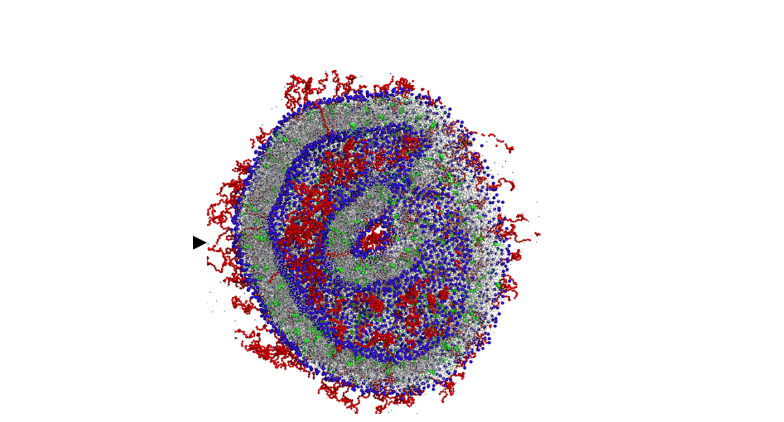
\includegraphics[width=\linewidth]{abstracts/txt/figures/sudip.png}  \caption{Self-assembled supramolecule for drug delivery.}  \end{center}  
    
        \textbf{References} \newline{}[1] Sarkar, S.; Chakraborty, S.; Roy, S. Phase Diagram of Self-Assembled Sophorolipid Morphologies from Mesoscale Simulations. J. Mol. Liq. 2018, 254, 198–207.\newline{}[2] Kulkarni, A.; Pandey, P.; Rao, P.; Mahmoud, A.; Goldman, A.; Sabbisetti, V.; Parcha, S.; Natarajan, S. K.; Chandrasekar, V.; Dinulescu, D.; Roy, S.; Sengupta, S.; et al. Algorithm for Designing Nanoscale Supramolecular Therapeutics with Increased Anticancer Efficacy. ACS Nano 2016, 10 (9), 8154–8168.\newline{}[3] Pandey, P. R.; Dhasaiyan, P.; Prasad, B. L. V; Roy, S. Structural Insight into Self Assembly of Sophorolipids: A Molecular Dynamics Simulation Study. Zeitschrift für Phys. Chemie 2016, 230 (5–7), 819–836 IF: 1.356.\newline{}[4] Dhasaiyan, P.; Pandey, P. R.; Visaveliya, N.; Roy, S.; Prasad, B. L. V. Vesicle Structures from Bolaamphiphilic Biosurfactants: Experimental and Molecular Dynamics Simulation Studies on the Effect of Unsaturation on Sophorolipid Self-Assemblies. Chem. Eur. J. 2014, 20 (21), 6246–6250.\newline{}[5] Kumar, M.; Patil, N. G.; Choudhury, C. K.; Roy, S.; Ambade, A. V; Kumaraswamy, G. Compact Polar Moieties Induce Lipid--Water Systems to Form Discontinuous Reverse Micellar Phase. Soft Matter 2015, 11 (27), 5417–5424.
    \end{abstract_online}
    